%Related Work/ Background/ Lit Review
\section{Related Work}
In general, grid generation is a name for any process that creates a grid.  
For example, the advancing-front algorithm advances boundaries into space 
to generate a grid \cite{lohner88}.  Other methods generate grids from 
iterative refinement or enrichment from initial, coarse 
configurations[cite].  Usually the benchmark for separating the two 
methods, generation and refinement, are the prioritization of grid quality 
and grid accuracy (both of these issues will be addressed later).  From a 
standard text \cite{thompson98}: One dimensional grids, or edge grids, 
\begin{quotation} \noindent ``...are created using a one-dimensional 
version of the standard grid generation procedure.  This ensures that 
point distribution and growth rates are fully compatible for optimal final 
grid quality.  For each edge or segment the point spacing is specified at 
both ends... Edge grid generation is then used to produce the point 
distribution...'' \end{quotation} An example of this can be seen below in Figure-\ref{EdgeGrid_HandbookOfGridGeneration} where the point spacing distributions are df1 and df2.

\begin{figure}[h!]
  \center{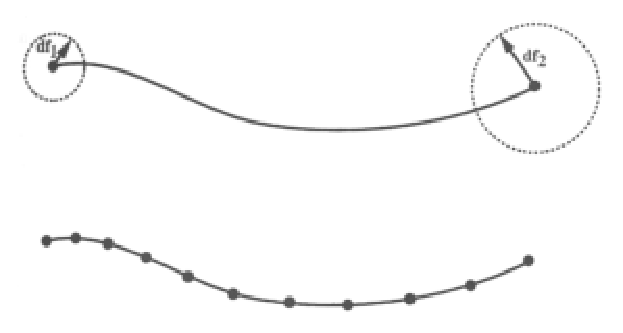
\includegraphics[width=0.8\textwidth]
    {Figures/EdgeGrid_HandbookOfGridGeneration.eps}}
  \caption{\label{EdgeGrid_HandbookOfGridGeneration} Caption}
\end{figure}

\noindent In the example above, the edge grid generation process produces good quality grids from the combination of geometric growth rates and smoothing.  However, the process requires input: point spacing values.  If the point spacing values are not appropriate then the geometry can be under and/or over sampled for the intended use.  That fact is not an indictment of the grid generation process, but instead implies that the final grid is heavily dependent on the inputs.  In addition, if some way of controlling the point spacing in the middle of a curve is not present, then more points could be wasted/omitted in an attempt to accurately represent geometry.

Instead of setting appropriate point spacing values and using common grid generation techniques, other efforts have gone into creating a locally or globally ``optimal'' edge grid.  Many names have been assigned to this particular task, but the underlying goal is very similar—represent a curve as accurately as possible—whatever that means for each application.  For example, \cite{laug04} first linearized the interface between curves in order to simplify the process of generating edge grids and surface grids on topologically adjacent patches.  Other ``geometry aware'' or ``curvature based'' approaches have been developed.  One such application is for discretizing curves for use in level set methods \cite{macklin06}.  Others include energy minimization \cite{hofer04}, curvature minimization \cite{zehiry10}, and angle minimization \cite{ebeida10}.

